\documentclass[a4paper]{article}

\usepackage[english]{babel}
\usepackage[utf8]{inputenc}
\usepackage{amsmath}
\usepackage{graphicx}
\usepackage[colorinlistoftodos]{todonotes}
\usepackage{algorithm} % http://ctan.org/pkg/algorithms
\usepackage{algpseudocode} % http://ctan.org/pkg/algorithmicx
\algnewcommand\algorithmicforeach{\textbf{for each}}
\algdef{S}[FOR]{ForEach}[1]{\algorithmicforeach\ #1\ \algorithmicdo}


\title{Homework 2 - The Exploration-Exploitation Dilemma}

\author{Henrique Gasparini Fiuza do Nascimento}

\date{\today}

\begin{document}
\maketitle

\begin{abstract}

In this report, we explore the exploration-exploitation dilemma for multi-armed bandits models on both simulated and real data, by implementing several algorithms to reduce the accumulative regret.

\end{abstract}

\section{Stochastic Multi-Armed Bandits on Simulated Data}
\label{sec:first_exercise}

\subsection{Bernoulli bandit models}

\textbf{Question 1}: For two different Bernoulli bandit problems (that you specify), with different complexity, compare the regret of Thompson Sampling with that of UCB1. Add Lai and Robbins’ lower bound on your plots.
\paragraph{•}
\textit{Answer}: we explored 3 problems, with different levels of difficulty.. We say that a problem is easy when the mean from the arm with the largest mean is significantly larger than the others.

\begin{description}
\item[Moderate problem] Bernoulli arms with parameters 0.3, 0.25, 0.2, 0.1. The problem complexity is 12.662 and the plot is at figure \ref{fig:Bernoulli_moderate_problem}.
\item[Difficult problem] Bernoulli arms with parameters 0.3, 0.29, 0.29, 0.29. The problem complexity is 124.367 and the plot is at figure \ref{fig:Bernoulli_difficult_problem}.
\item[Easy problem] Bernoulli arms with parameters 0.9, 0.15, 0.10, 0.05. The problem complexity is 1.349 and the plot is at figure \ref{fig:Bernoulli_easy_problem}.

\end{description}

\begin{figure}
\centering
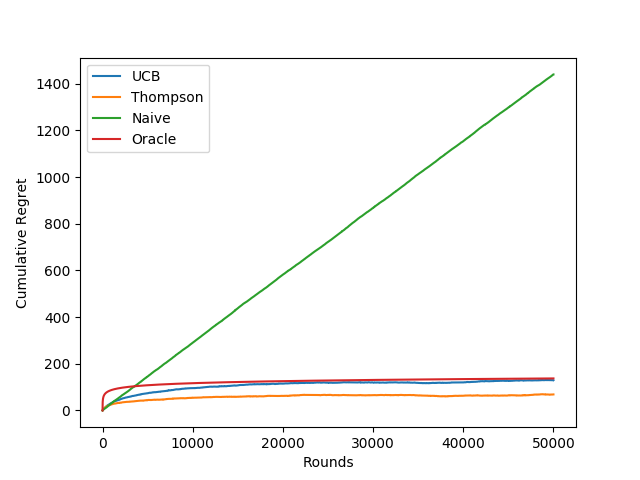
\includegraphics[width=1\textwidth]{../img/Regret curves for Bernoulli moderate problem.png}
\caption{\label{fig:Bernoulli_moderate_problem}}
\end{figure}

\begin{figure}
\centering
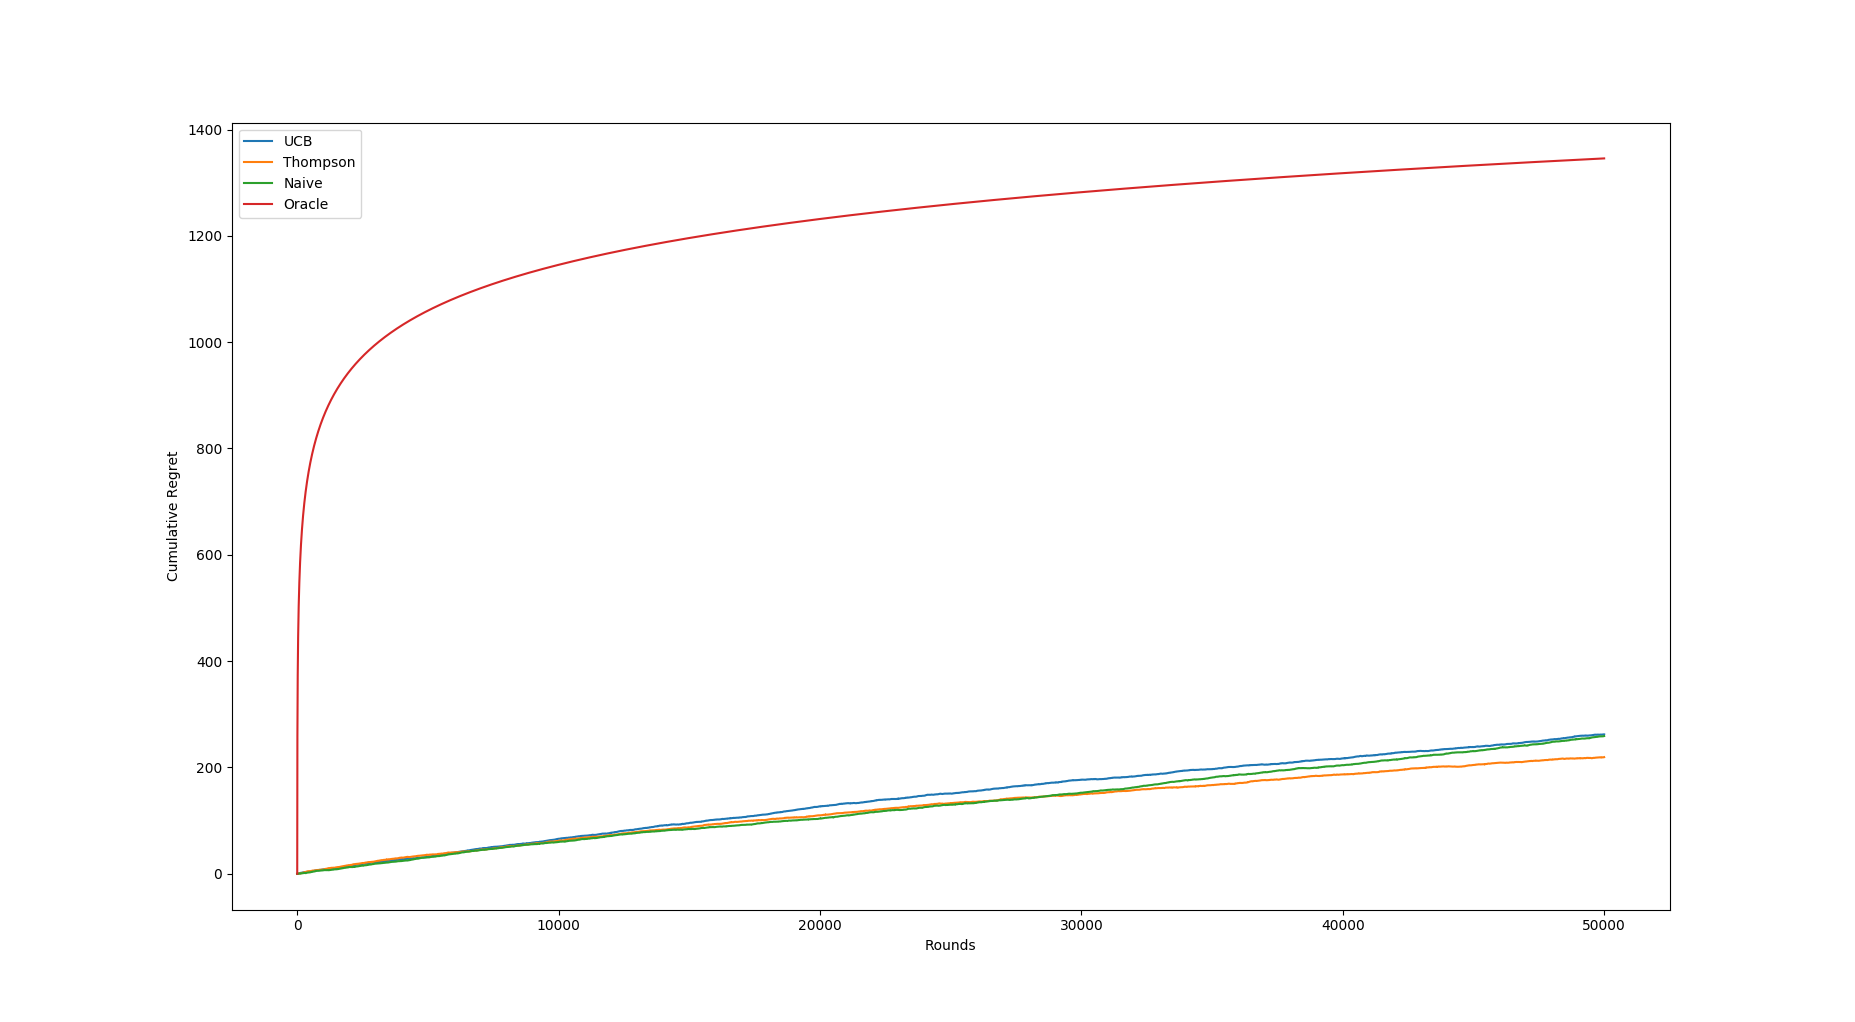
\includegraphics[width=1\textwidth]{../img/Regret curves for Bernoulli difficult problem.png}
\caption{\label{fig:Bernoulli_difficult_problem}}
\end{figure}

\begin{figure}
\centering
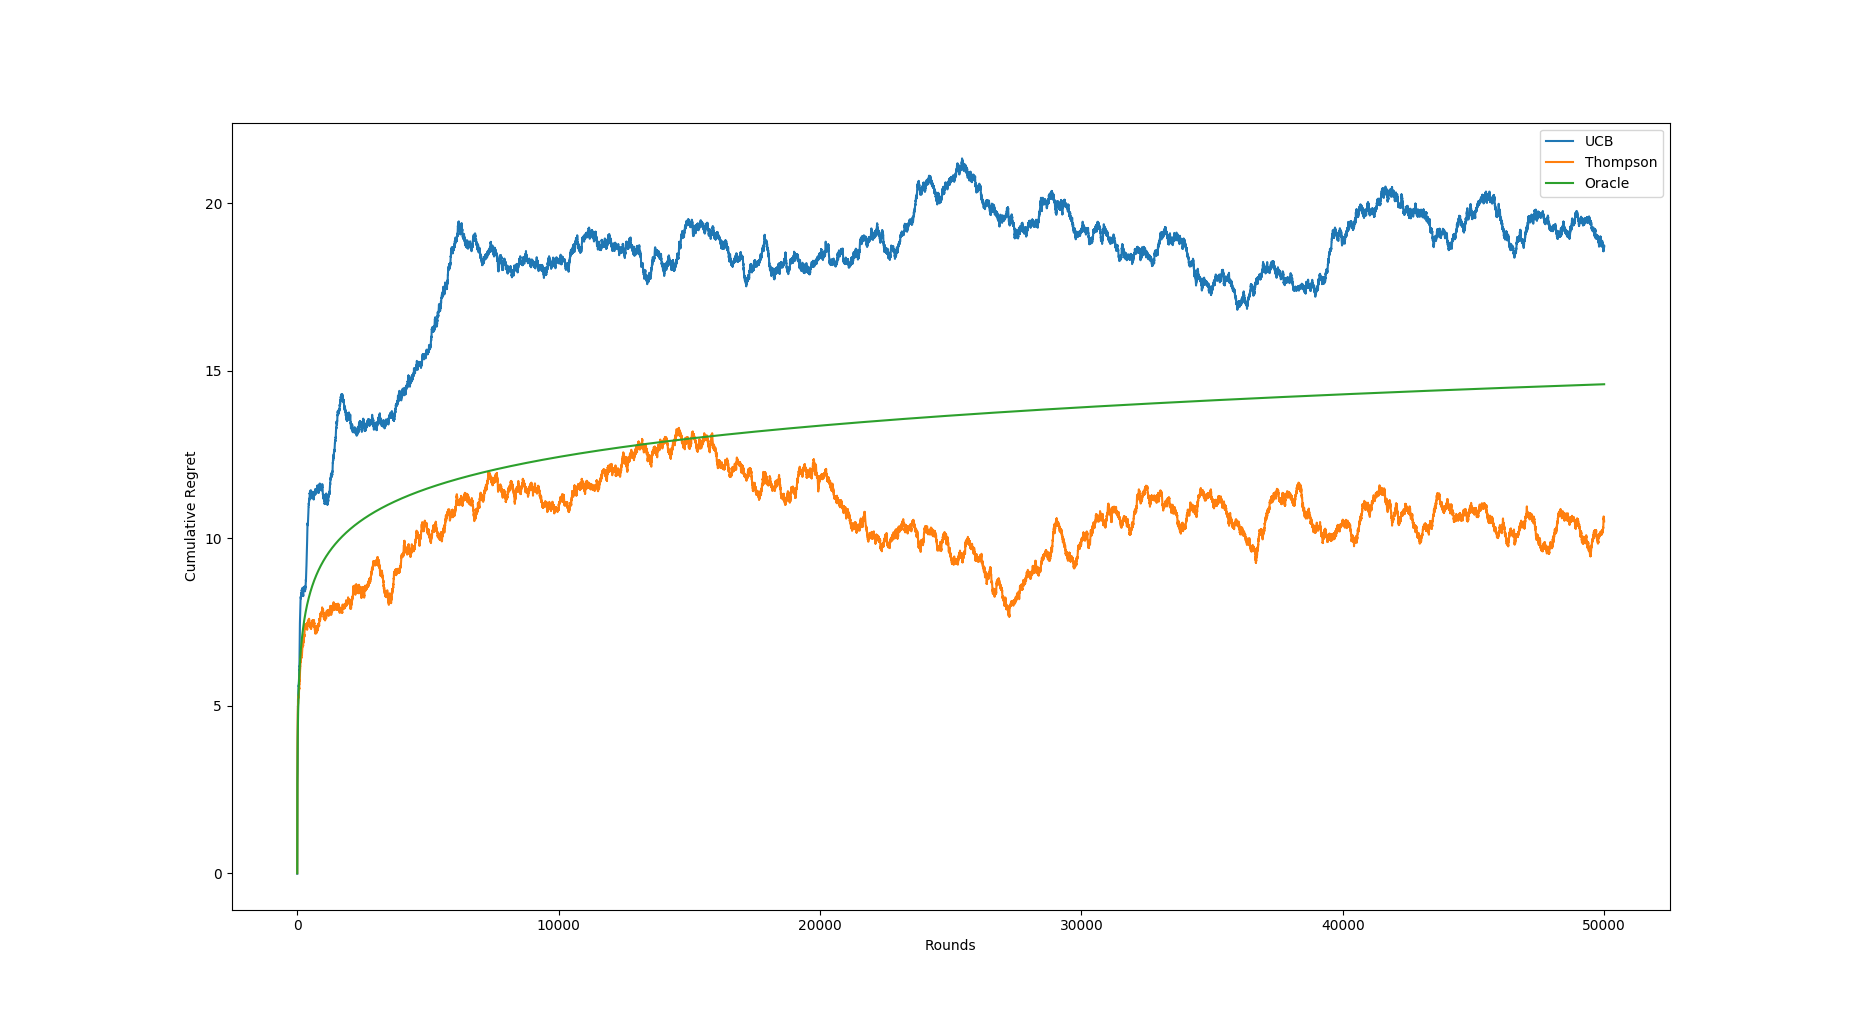
\includegraphics[width=1\textwidth]{../img/Regret curves for Bernoulli easy problem.png}
\caption{\label{fig:Bernoulli_easy_problem}}
\end{figure}

From looking at these plots, we can observe that the naive strategy is considerably worse than the others and that Thompson sampling is the most efficient. We could also say that the convergence to the Lai and Robbins lower bound is more rapidly attained in easier problems.

For the UCB1 algorithm, we used $\rho = 0.2$ to weight the uncertainty, which is the value suggested in the course lectures and produced good results.

\subsection{Non-parametric bandits (bounded rewards)}

\textbf{Question 2}: Describe the proposed implementation of Thompson Sampling and present a regret curve in a bandit model that you specify. Does the notion of complexity still make sense? Suggestion: [Burnetas and Katehakis, 1996].
\paragraph{•}
\textit{Answer}:
The reformulated Thompson Sampling algorithm is described by Agrawal and Goyal\cite{AdaptedThompson} as in Algorithm 1. The fifth line (which is highlighted) is the adaptation that was made for problems in which the reward lies in the continuous interval $[0, 1]$.

\begin{algorithm}[h]
	\caption{Thompson Sampling for general stochastic bandits}
	$S_i=0, F_i=0$.
	\ForEach{$t=1, 2, \ldots,$}
		\State For each arm $i=1,\ldots, N$, sample $\theta_i(t)$ from the $\Beta(S_i+1, F_i+1)$ distribution.
		\State Play arm $i(t) := \arg \max_i \theta_i(t)$ and observe reward $\tilde{r}_t$.
        \State \textbf{Perform a Bernoulli trial with success probability $\tilde{r}_t$ and observe outp$r_t$.}
		\State If $r_t=1$, then $S_{i}=S_i+1$, else $F_i=F_i+1$.
	\EndFor
\end{algorithm}

The notion of complexity still exists and in explained in Burnetas and Katehakis \cite{Complexity}, whose theorem 1 proves an equivalent asymptotic lower bound.

For an arm $a$ following a parametric distribution $f_a(\cdot; \theta_a)$, we first define $I(\theta_a, \theta_a^{'}) = \mathbb{E}_{\theta_a}[\log (\dfrac{f_a(Y_a; \theta_a)}{f_a(Y_a; \theta_a^{'})})]$. Then we can define $K_a(\theta) = \inf(I(\theta_a, \theta_a^{'}) \| \mu_a(\theta_a^{'}) > \mu^{*})$.

The complexity of the problem is then given by:

\begin{center}
    $\sum\limits_{a \in arms} \dfrac{\mu^* - \mu_a}{K_a(\theta)}$
\end{center}

For the sake of this assignment, we opted not to implement this formula, as it would require solving a couple optimization with constraints problems. Had we more time and actually were we asked to compute it in the exercise statement, it sure could be done.

We simulated the adapted Thompson sampling algorithm in a model consisted of:

\begin{enumerate}
    \item \textit{A Bernoulli arm}: $p = 0.3$, mean $0.3$
    \item \textit{A Beta distribution arm}: $a = 0.5$, $b = 0.5$, mean $0.5$
    \item \textit{A Beta distribution arm}: $a = 1$, $b = 3$, mean $0.25$
    \item \textit{An Exponential distribution arm}: $L = 1.0$, mean $0.418$
    \item \textit{A arm with a distribution with finite support}: $X = [0., 0.1, 0.5, 0.8]$, $P = [0.2, 0.3, 0.4, 0.1]$, mean $0.31$
\end{enumerate}

We plotted the regret of each of the sampling algorithms in figure \ref{fig:non_parametric_problem}. For the plotted oracle curve, we computed the problem complexity using the same formula we used for Bernoulli bandit models just to have some weak reference.

\begin{figure}
\centering
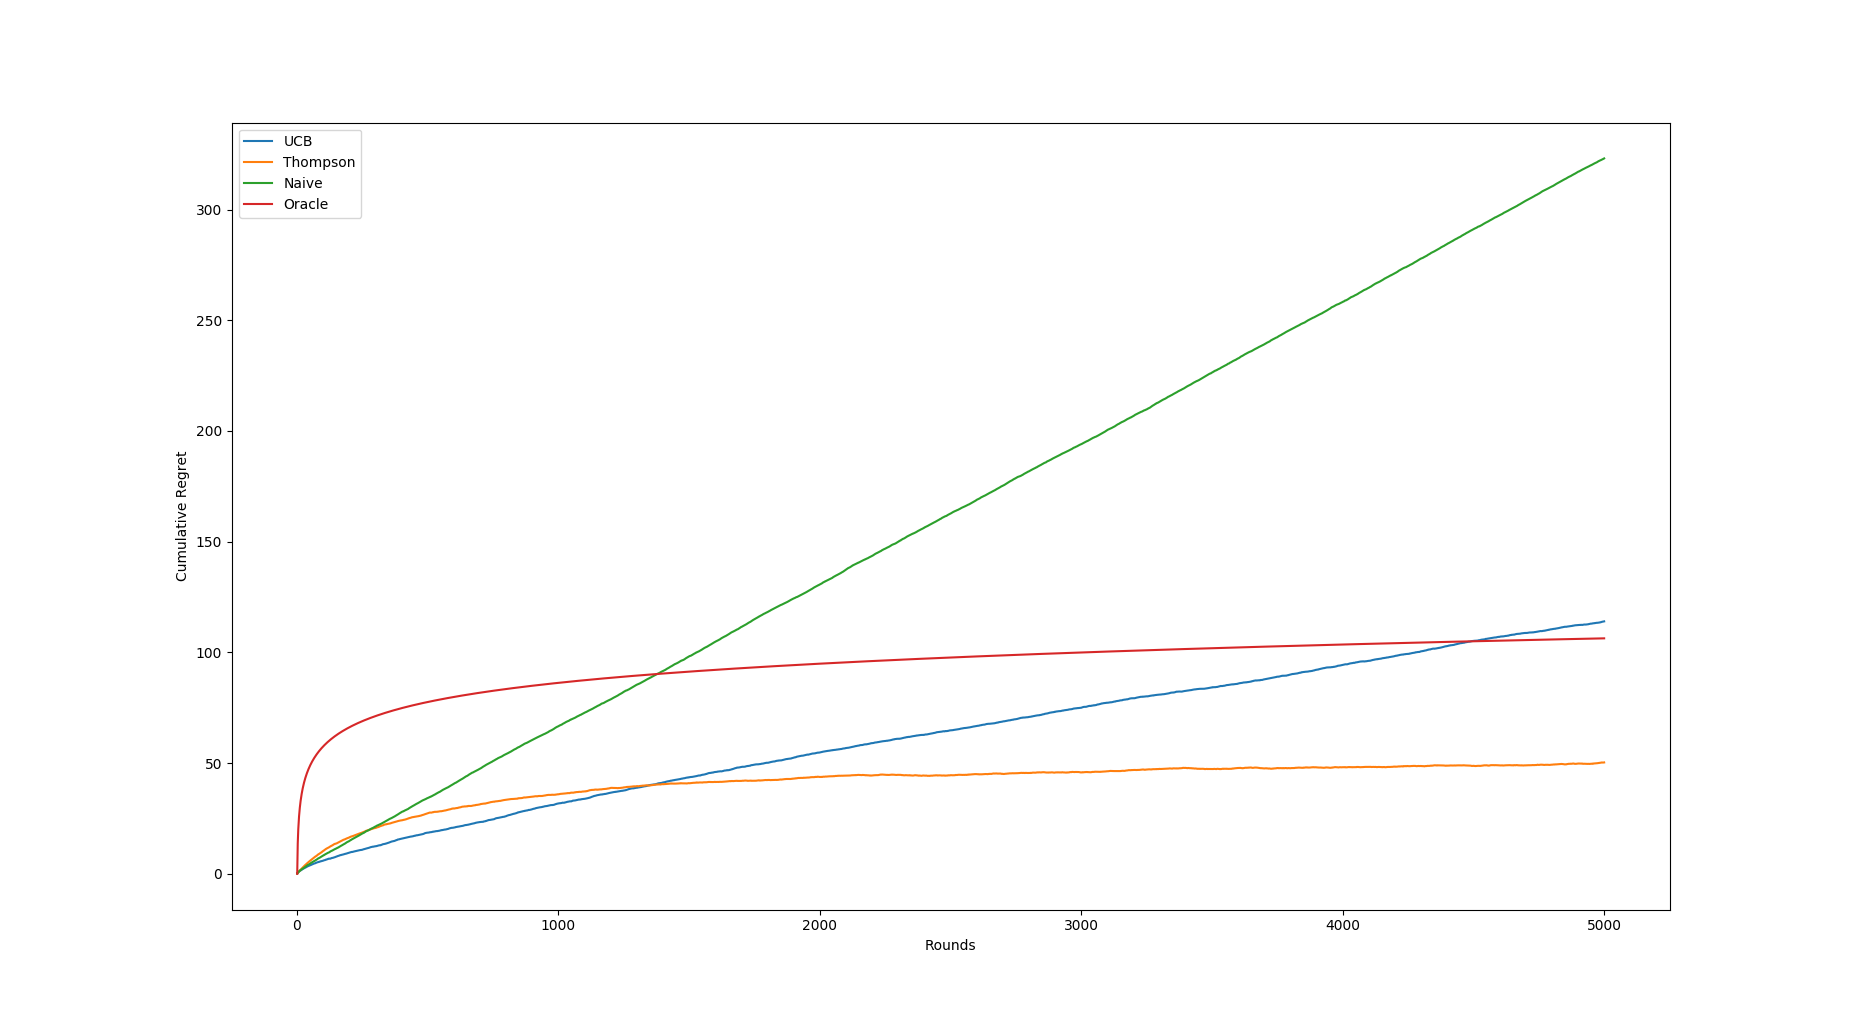
\includegraphics[width=1\textwidth]{../img/Regret curves for non parametric problem.png}
\caption{\label{fig:non_parametric_problem}}
\end{figure}

\section{Linear Bandit on Real Data}
\label{sec:second_exercise}

\textbf{Question 3}: Implement the LinUCB algorithm for the provided MovieLens problem. Compare the performance against the following algorithms (consider a horizon T = 6000):
\begin{itemize}
    \item \textbf{random}: A random policy always chooses one of the candidate movies from the pool with equal probability.
    \item \textbf{$\epsilon$-greedy}: it estimates each movie’s rating; then it chooses a random movie with probability $\epsilon$ and chooses the movie of the highest rating estimate with probability $1 - \epsilon$.
\end{itemize}
Play with the parameters of each algorithm and report your choice. Remember to average the regret on multiple simulations as done for the Bernoulli exercise.

\paragraph{•}
\textit{Answer}: We implemented three classes which implement, respectively, the random, $\epsilon$-greedy, and LinUCB algorithms: \texttt{RandomStrategy}, \textt{EpsilonGreedyStrategy}, and \textt{LinUCBStrategy}.

They all implement two important methods:

\begin{itemize}
    \item \textbf{select}: determines which arm to select in a time $t$.
    \begin{description}
        \item[Random] Each arm has equal probability of being selected
        \item[$\epsilon$-greedy] The arm with the highest estimated expected reward ($\hat{\theta}^T \phi_a$) is selected with probability $1 - \epsilon$. A random arm is selected with probability $\epsilon$
        \item[LinUCB] The arm with the highest upper bound estimated expected reward is selected. The upper bound estimation of an arm is computed as the estimated expected reward ($\hat{\theta}^T \phi_a$) plus an error $\beta_a = \alpha_t \cdot \sqrt{\phi_a^T(Z_t^T Z_t + \lambda I)^{-1}\phi_a}$. The matrix $Z_t$ consists of the stacked $\phi_a$s of previously selected arms. The confidence $\alpha_t$ can be just a constant or may vary over time following an expression like $\alpha_t = \alpha * \sqrt{\log t}$.
    \end{description}
    \item \textbf{update}: updates the history of actions and rewards, as well as the estimated user vector $\hat{\theta} = (Z_t^T Z_t + \lambda I)Z_t^T y_t$, in which $y_t$ is the vector of past rewards.
\end{itemize}


\textbf{Hyper-parameter tuning}: we looked for hyper-parameters that minimized the accumulated regret for each of those strategies and found that $\epsilon = 0.01$, and $\alpha = 0.3$ produced the smaller accumulated regrets in average by the end of the simulations. We also observed that using constant $\alpha_t$ produced similar results to when we used the logarithmically increasing $\alpha_t$.

\textbf{Plots}: we plotted the average over 20 simulations of both the squared difference between the estimated $\theta$ and the real $\theta$ and the accumulated regret over an horizon $T = 6000$ at figure \ref{fig:real_data}.

\begin{figure}
\centering
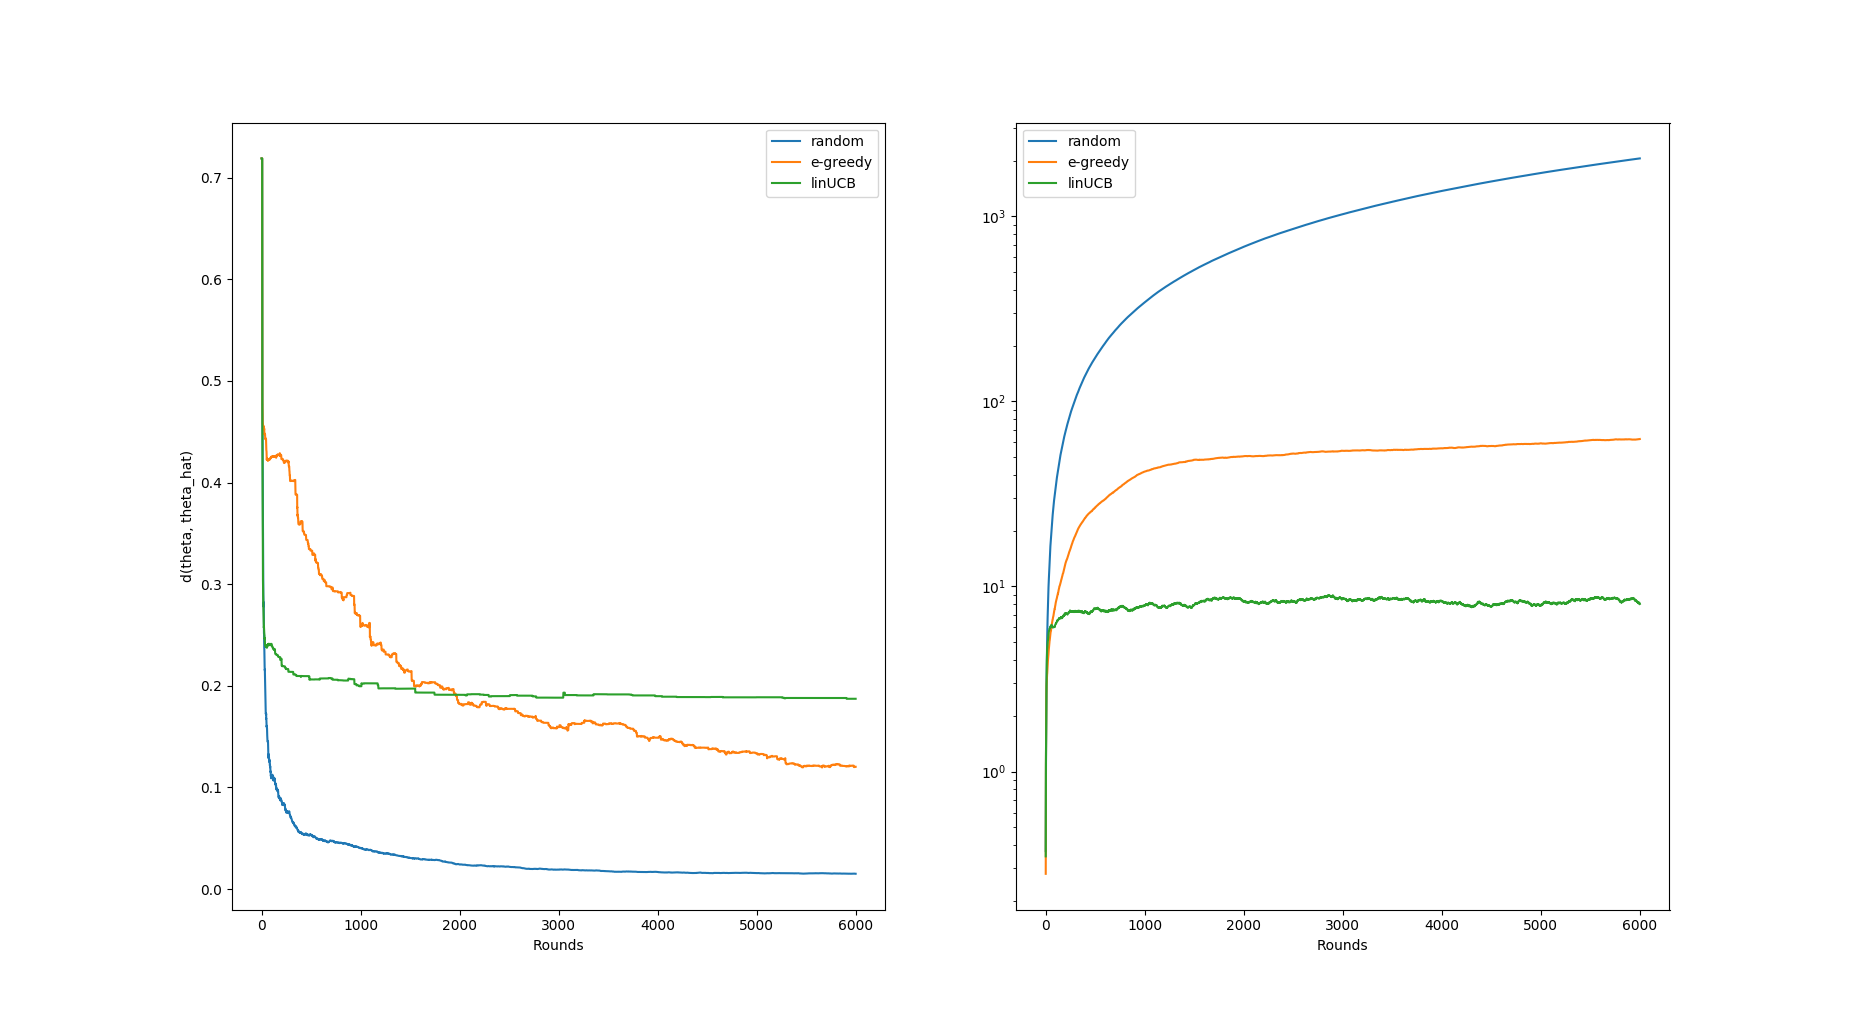
\includegraphics[width=1\textwidth]{../img/Regret curves for linear bandit model on real data.png}
\caption{\label{fig:real_data}}
\end{figure}

\textbf{Convergence and asymptotic analysis}: When looking at the plots, one can observe an almost stationary accumulated regret which grows very slowly (as we know and mentioned before, it grows at least logarithmically). That happens because the algorithm very often correctly discovers the arm with the optimal expected reward after a certain time horizon. However, the estimated $\theta$ does not necessarily converge to the real $\theta$. This happens in particular for the LinUCB algorithm.

In fact, the optimal arm is found so quickly that the attempts on others arm are not numerous enough to allow an accurate estimate of $\theta$. To give one reason for that, for example, it is reasonable to say that some arms may never pulled. If the number of arms that are pulled at least once is smaller than the number of features then the solution for optimizing $\theta$ is not unique (we will have a "linear equations system" with less equations than variables).

\textbf{Future implementation optimization}: as a next step for the implementation, we could reduce the total simulation time by reducing the number of operations required to compute $(Z_t^T Z_t  + \lambda I)^{-1}$ at each iteration. In fact, one can write $Z_{t+1}^T Z_{t+1}  + \lambda I = Z_t^T Z_t + \phi_{a_{t+1}}\phi_{a_{t+1}}^T + \lambda I$ and then apply Sherman–Morrison's inversion formula\cite{InvertSum}: $(A + uv^T)^{-1} = A^{-1} - \dfrac{A^{-1}uv^TA^{-1}}{1 + v^TA^{-1}u}$, for $A = Z_t^T Z_t$, $u = v = \phi_{a_{t+1}}$. This would reduce the time to compute the inverse from $O(f^3)$ to $O(f^2)$ (where we denote $f$ the number of features), which can be a substantial gain if the number of features is big. In our case, $f= 8$ is quite small, so the impact probably would be less significant.


\bibliographystyle{unsrt}
\bibliography{bib}

\end{document}
